% !TeX spellcheck = ru_RU
% !TEX root = vkr.tex

\section{Обзор}
В этом разделе будут введены необходимые для понимания работы термины и  понятия.
\subsection{Деревья квадрантов}
Деревья квадрантов~--- рекурсивная структура данных для представления разряженных матриц. Данная матрица приводится до квадратной с размером, равным степени двойки, далее,если все элементы матрицы равны, то дерево представляется в виде пары значения и размера и будет называться листом дерева, в ином случае разделяется на четыре равные части~--- дочерние узлы (квадранты), которые тоже представляют собой деревья квадрантов. Так происходит до тех пор, пока каждый узел не дойдёт до листа. Таким образом, строится дерево в привычном для математиков понимания этого слова. визуальное представление этого процесса представлено на рис. \ref{qmatrix} и рис. \ref{qtree1}. Эта структура позволяет \enquote{сжимать} повторяющиеся и находящиеся близко данные в один узел.

\begin{figure}[h!]
    \centering
    \resizebox{0.45\textwidth}{!}{
        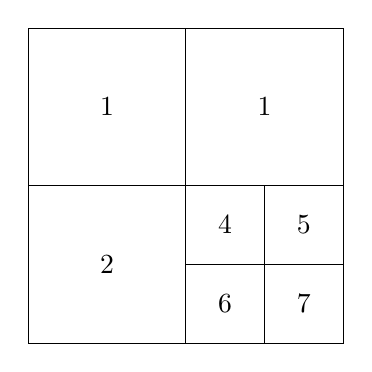
\begin{tikzpicture}
            \draw (1, 1) rectangle (3, 3);
            \node at (2, 2){2};
            \draw (1,3) rectangle (3, 5);
            \node at (2, 4) {1};
            \draw (3, 3) rectangle (5, 5);
            \node at (4, 4) {1};
            \draw (3, 1) rectangle (4, 2);
            \node at (3.5, 1.5) {6};
            \draw (3, 2) rectangle (4, 3);
            \node at (3.5, 2.5) {4};
            \draw (4, 1) rectangle (5, 2);
            \node at (4.5, 1.5) {7};
            \draw (4, 2) rectangle (5, 3);
            \node at (4.5, 2.5) {5};
        \end{tikzpicture}
    }
    \caption{Квадратная матрица, разделенная на квадранты}
    \label{qmatrix}
\end{figure}
\begin{figure}[h!]
    \centering
    \Tree [.A
            [.{Leaf(1, 2)}  ]
            [.{Leaf(1, 2)}  ]
            [.{Leaf(2, 2)}  ]
            [.SE
                    [.{Leaf(4, 1)}  ]
                    [.{Leaf(5, 1)}  ]
                    [.{Leaf(6, 1)}  ]
                    [.{Leaf(7, 1)}  ]
            ]
        !\qsetw{0.5cm}
    ]
    \caption{Изображение дерева квадрантов в виде дерева}
    \label{qtree1}
\end{figure}

\subsection{Слияние ядер}
% Слияние ядер (англ. \textit{kernel fusion})
Требует уточнения
\subsection{Метапрограммирование}
Метапрограммирование~--- это процесс создание программ, которые в ходе своего выполнения генерируют другие программы. В контексте поставленной задачи оно было необходимо, так как нужно было
\begin{enumerate}[label=(\alph*)]
    \item генерировать функции в зависимости от данных, поданных пользователем;
    \item размер этого кода был довольно большим, но при этом обладал вполне регулярной структурой.
\end{enumerate}
В языке \Haskell{} есть встроенная библиотека с обширной и доступной документацией: \Th{}, которая позволяет генерировать код на \Haskell{} во время компиляции. При этом возможно использовать как синтаксис источника, так и более строгий специализированный для генерации кода.
